	\chapter{Robot Performance/Animation}
		The way that I designed the development environment for the hexapod, I am able to animate the routine to the music using the open-source 3D modeling and animation software, Blender.\\
        
        \section{Animation}
        
          To give you the best overall idea of what the process of animating the robot looks like, I've compiled a stopmotion video of me animating a movement. This particular movement was for States, and I was animating the robot stepping off a raised platform, onto the ground. This took around 2 hours for me to animate.\\

          \url{https://www.youtube.com/watch?v=o0-15CS6urg}\\

          All things considered animation isn't the most time consuming activity, but I might venture to say that it is the most irritating. Often you are listening to the same music over and over, and doing very repetitive tasks. Often you have to delete half an hours worth of work at a time. It's not uncommon to throw away several seconds of content (which could have taken hours to create).\\

          You can do many things when animating that won't work in real life - you can make the robot jump in Blender, but that doesn't mean the robot will jump in real life. You need to have a good sense of how the robot works, physically, to be able to animate it. This is not all bad though - if you are familiar with what the robot will do in regards to how you animate it in Blender, you can achieve some pretty amazing results that you wouldn't normally be able to achieve if you animated the robot conventionally.\\

          The soundtrack has to be fully created before starting animation, as I animate to the music. To do this I add the soundtrack to the timeline in Blender, allowing me to hear the audio whilst I'm animating, allowing me to animate to the music.\\

          \centerline{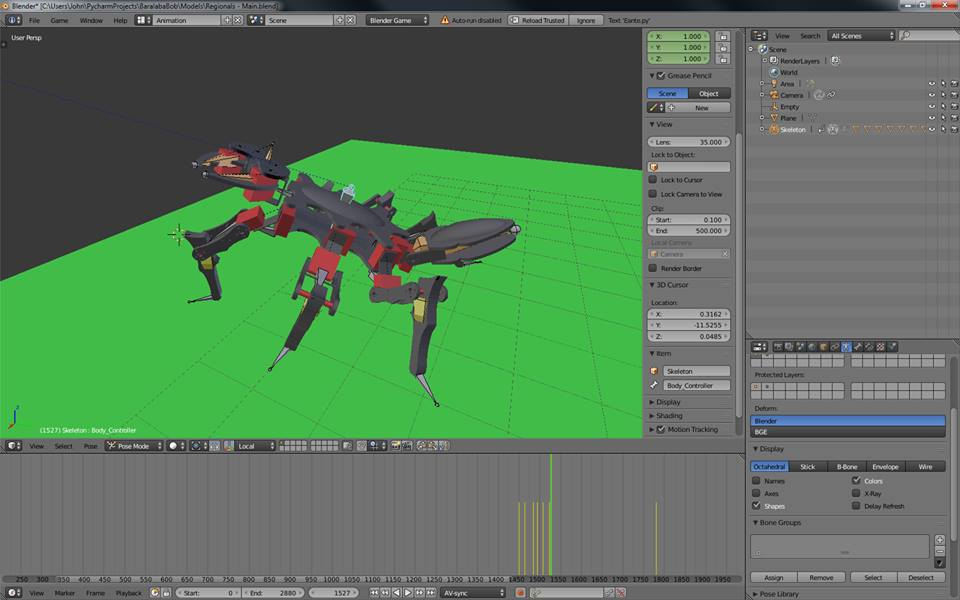
\includegraphics[width=\linewidth]{images/animation}}
          \vspace{10pt}
          \centerline{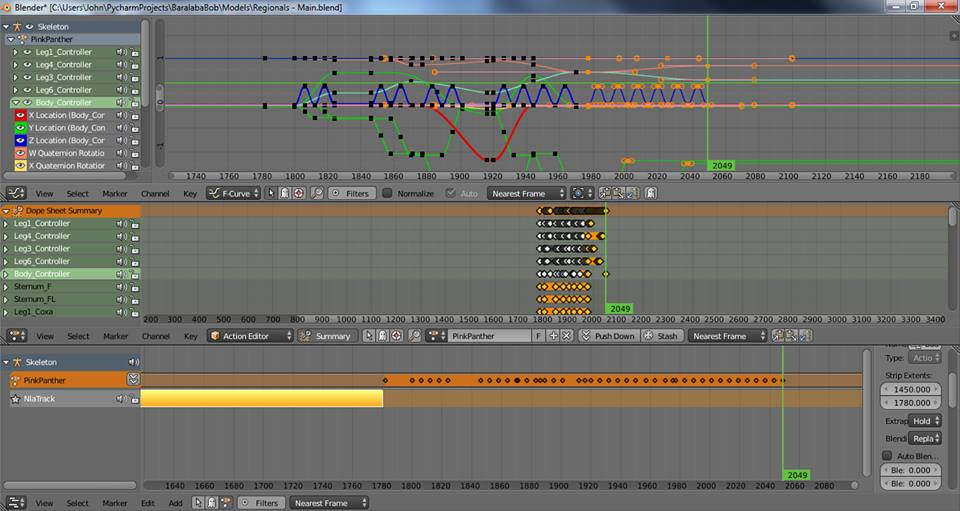
\includegraphics[width=\linewidth]{images/graph_editor}}
          \vspace{10pt}
          
          
         \index{unique}
		\section{Performance}
        	Before animating the routine for \index{regionals}Regionals, I had thought of a lot of movements which I could put to music - allowing me to develop them quickly. For \index{states}States I hadn't thought of movements - I was animating and making up movements on the fly.\\
            
			Some considerations in the development of the \index{robot}robot's routine is making sure I use as much of the \index{floor space}floor space as possible, having lots of \index{unique movements}unique movements to maintain interest, making sure the movements fit the audio, and ensuring that the movements aren't straining the robot \index{motor failure} (causing motor failure).\\
            
            \textit{\textbf{Also see: }\hyperref[motor_failure]{Motor Failure}}
            
            It's very difficult to walk the robot around the entire floor space, as it takes a while to have the robot walk anywhere. Part of this is my not wanting to strain the robot by having it walk fast, but as time goes on I get more and more adventurous with how far I push the robot. The problem of \index{movement speed}movement speed still presents itself.\\
            
            One of the sub-difficulties is that turning the robot is very slow. It takes a minimum of 3-4 individual turn sequences on the robot to turn a full 90 degrees, each turn taking 0.5-2 seconds. Multiply 4 by 2 seconds, and you quickly run into a very time consuming movement, at 8 seconds - and that's just to turn 90 degrees. I prefer to have the robot walk sideways, than turning sideways and then walking in that direction. The advantage of a legged base is that you don't have to face the direction you walk, so you can do this.\\
            
            Having unique movements to provide interest isn't particularly difficult to create, but it is often difficult to animate and time consuming to integrate into the routines. It often takes many hours of continuous effort to animate a single 10-15 second segment.\\
            
            

        
        
    	